\documentclass{beamer}

\usepackage{tikz}

\title{Basic Trigonometric Identities and Equations}


\date{}
\begin{document}

\frame{\titlepage}

\begin{frame}{Trigonometric Identities}
    \begin{description}
        \item[Quotient Identities] {\begin{equation*}
            \tan{\theta}=\frac{\sin{\theta}}{\cos{\theta}}\;\;\;\;\;
            \cot{\theta}=\frac{\cos{\theta}}{\sin{\theta}}
            
        \end{equation*}}
        
        \item[Reciprocal Identities] {\begin{equation*}
            \sin{\theta}=\frac{1}{\csc{\theta}}\;\;\;\;\;
            \cos{\theta}=\frac{1}{\sec{\theta}}\;\;\;\;\;
            \tan{\theta}=\frac{1}{\cot{\theta}}
        
        \end{equation*}}
        
        \item[Pythagorean Identities] {\begin{equation*}
            \alert{\sin{\theta} ^ 2 + \cos{\theta} ^ 2 = 1}\;\;\;
            \alert{\tan{\theta} ^ 2 + 1 = \sec{\theta} ^ 2}\;\;\;
            \alert{\cot{\theta} ^ 2 + 1 = \csc{\theta} ^ 2}
\end{equation*}
        \begin{equation*}    
            \sin{\theta} ^ 2 = 1 - \cos{\theta} ^ 2\;\;\;
            \tan{\theta} ^ 2 = \sec{\theta} ^ 2 - 1\;\;\;
            \cot{\theta} ^ 2 = \csc{\theta} ^ 2 - 1
            
        \end{equation*}}
    \end{description}
\end{frame}





\begin{frame}{Using the identities you now know, find the trig value.}
\begin{columns}
 \column{0.5\textwidth}
    1.) If $\cos{\theta} = 3/4$, find $\sec{\theta}$
    \begin{equation*}
        \sec{\theta}=\frac{1}{\cos{\theta}}=\frac{1}{\frac{3}{4}}=\frac{4}{3}
    \end{equation*}
 \column{0.5\textwidth}
    2.) If $\cos{\theta} = 3/5$, find $\csc{\theta}$
    \begin{equation*}
        \sin{\theta} ^ 2 + \cos{\theta} ^ 2 = 1
    \end{equation*}
    \begin{equation*}
        \sin{\theta} ^ 2 + (\frac{3}{5}) ^ 2 = 1
    \end{equation*}
\end{columns}

\end{frame}


\begin{frame}{Simplify each expression}
\begin{columns}
 \column{0.2\textwidth}
    1.) If $\cos{\theta} = 3/4$, find $\sec{\theta}$
    \begin{equation*}
        \sec{\theta}=\frac{1}{\cos{\theta}}
    \end{equation*}
 \column{0.4\textwidth}
    2.) If $\cos{\theta} = 3/5$, find $\csc{\theta}$
    \begin{equation*}
        \sin{\theta} ^ 2 + \cos{\theta} ^ 2 = 1
    \end{equation*}
    \begin{equation*}
        \sin{\theta} ^ 2 + (\frac{3}{5}) ^ 2 = 1
    \end{equation*}
    
 \column{0.4\textwidth}
    2.) If $\cos{\theta} = 3/5$, find $\csc{\theta}$
    \begin{equation*}
        \sin{\theta} ^ 2 + \cos{\theta} ^ 2 = 1
    \end{equation*}
    \begin{equation*}
        \sin{\theta} ^ 2 + (\frac{3}{5}) ^ 2 = 1
    \end{equation*}
\end{columns}

\end{frame}



\begin{frame}{Example}
    Simplify:
    \begin{enumerate}
        \item [a)] csc
    \end{enumerate}
\end{frame}




\begin{frame}{Practice}
    \centering
    \begin{tabular}{|c|c|c|c|}
         \hline
         $sec\theta$&$sec\theta$ &$sec\theta$ &$sec\theta$ \\
         \hline
         $sec\theta$&$sec\theta$ &$sec\theta$ &$sec\theta$ \\
         \hline
    \end{tabular}
\end{frame}


\newlength{\R}\setlength{\R}{2.7cm}

\begin{frame}{}
    \centering
    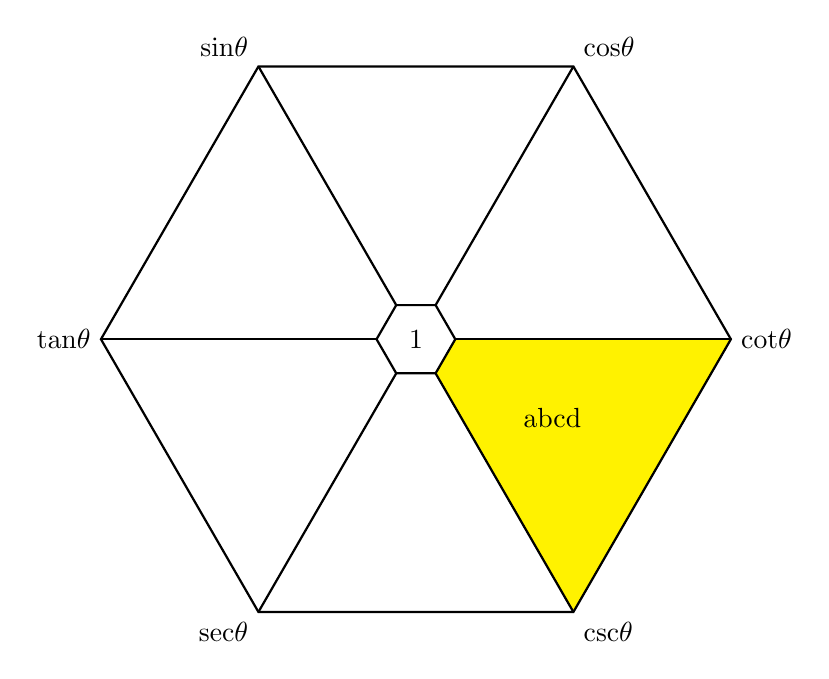
\begin{tikzpicture}


    
    \draw [fill=yellow] (300:4) -- (0:4) -- (0:0.5) -- (300:0.5) -- cycle;
    \draw node at (330:2) {abcd};


    \draw [thick] (300:4) 
    node[anchor = north west]{csc$\theta$} 
    -- (0:4) node[anchor = west] {cot$\theta$} 
    -- (60:4) node[anchor = south west] {cos$\theta$} 
    -- (120:4) node[anchor = south east]{sin$\theta$} 
    -- (180:4) node[anchor = east]{tan$\theta$} 
    -- (240:4) node[anchor = north east]{sec$\theta$} 
    -- cycle;

    \draw [thick] (300:0.5)  -- (0:0.5) -- (60:0.5) -- (120:0.5) -- (180:0.5) -- (240:0.5) -- cycle;

    \draw [thick] (300:0.5) -- (300: 4);
    \draw [thick] (0:0.5) -- (0: 4);
    \draw [thick] (60:0.5) -- (60: 4);
    \draw [thick] (120:0.5) -- (120: 4);
    \draw [thick] (180:0.5) -- (180: 4);
    \draw [thick] (240:0.5) -- (240: 4);
    \draw node at (0:0) {1};
    
    
    \end{tikzpicture}
\end{frame}
\end{document}